\newcommand{\selector}[0]{[~S~\Rightarrow~y;~BE~] \lolli HE}
\newcommand{\comprehension}[0]{\{~\widehat{x};~BE;~SH~\}}
\newcommand{\aggregate}[0]{[~A~\Rightarrow~y;~\widehat{x};~BE;~SH_1;~SH_2~]}

Linear Meld (LM) is a logic programming language that offers a declarative and structured way to manage state.
A program consists of a database of facts and a set of derivation rules. The database includes persistent
and linear facts. Persistent facts cannot be deleted, while linear facts can be asserted and retracted.

The dynamic (or operational) semantics of LM are identical to Datalog.
Initially, we populate the database with the program's axiom facts and then determine which derivation rules can be applied by using the current database. Once a rule is applied, we derive new facts, which are then added to the database.
If a rule uses linear facts, they are retracted from the database.
The program stops when \emph{quiescence} is achieved, that is, when rules no longer apply.

Each fact is a predicate on a tuple of \emph{values}, where the type of the predicate prescribes the types of the arguments.
LM rules are type-checked using the predicate declarations in the header of the program. LM has a simple type system that includes types such as
\emph{node}, \emph{int}, \emph{float}, \emph{string}, \emph{bool}. Recursive types such as \emph{list X} and \emph{pair X; Y} are
also allowed.
Each rule in LM has a defined priority that is inferred from its position in the source file.
Rules at the beginning of the file have higher priority. We consider all
the new facts that have been not considered yet to create a set of \emph{candidate rules}.
The set of candidate rules is then applied (by priority) and updated as new facts are derived.

\subsection{Example}

We now present an example LM program in Fig.~\ref{code:btree_replace} that implements the key update operation for a binary tree
represented as a key/value dictionary.
We first declare all the predicates (lines 1-4), which represent the kinds of facts we are going to use.
Predicate \texttt{left/2} and \texttt{right/2} are persistent while \texttt{value/3} and \texttt{replace/3} are linear.
The \texttt{value/3} predicate assigns a key/value pair to a binary tree node and the \texttt{replace/3} predicate
represents an update operation that updates the key in the second argument to the value in the third argument.


{\scriptsize
\begin{figure}[h]
   \vspace{-0.5\intextsep}
\scriptsize\begin{Verbatim}[numbers=left]
type left(node, node).
type right(node, node).
type linear value(node, int, int).
type linear replace(node, int, int).

replace(A, K, New), value(A, K, Old)
   -o value(A, K, New). // we found our key

replace(A, RKey, RValue), value(A, Key, Value), !left(A, B), RKey < Key
   -o value(A, Key, Value), replace(B, RKey, RValue). // go left

replace(A, RKey, RValue), value(A, Key, Value), !right(A, B), RKey > Key
   -o value(A, Key, Value), replace(B, RKey, RValue). // go right

// binary tree configuration
value(@3, 3, 3). value(@1, 1, 1). value(@0, 0, 0).
value(@2, 2, 2). value(@5, 5, 5). value(@4, 4, 4).
value(@6, 6, 6).
!left(@1, @0). !left(@3, @1). !left(@5, @4). 
!right(@1, @2). !right(@3, @5). !right(@5, @6).

replace(@3, 6, 7). // replace value of key 6 to 7
\end{Verbatim}
\vspace{-0.5\intextsep}
\caption{Binary tree dictionary: replacing a key's value.}
  \label{code:btree_replace}
  \vspace{-0.5\intextsep}
\end{figure}
}

The algorithm uses three rules for the three cases of updating a key's value: the first rule performs the update
(lines 6-7); the second rule recursively picks the left branch for the update operation (lines 9-10); and the third
rule picks the right branch (lines 12-13).
The axioms of this program are presented in lines 15-22 and they describe the initial binary tree configuration,
including keys and values. By having the \texttt{update(@3, 6, 7)} axiom instantiated at the root node $@3$, we intend to
change the value of key 6 to 7.
Note that when writing rules or axioms, persistent facts are preceded with a \texttt{!}.

Figure~\ref{fig:btree_trace} represents the trace of the algorithm. Note that the program database is partitioned
by the tree nodes using the first argument of each fact. In Fig.~\ref{fig:btree_trace}a we present the database
filled with the program's axioms. Next, we follow the right branch using rule 3 since $6 > 3$ (Fig.~\ref{fig:btree_trace}b).
We then use the same rule again in Fig.~\ref{fig:btree_trace}c where we finally reach the key 6. Here, we apply rule 1 and
\texttt{value(@6, 6, 6)} is updated to \texttt{value(@6, 6, 7)}.

\begin{figure}[h]
   \vspace{-0.75\intextsep}
        \centering
        \begin{subfigure}[b]{0.5\textwidth}
                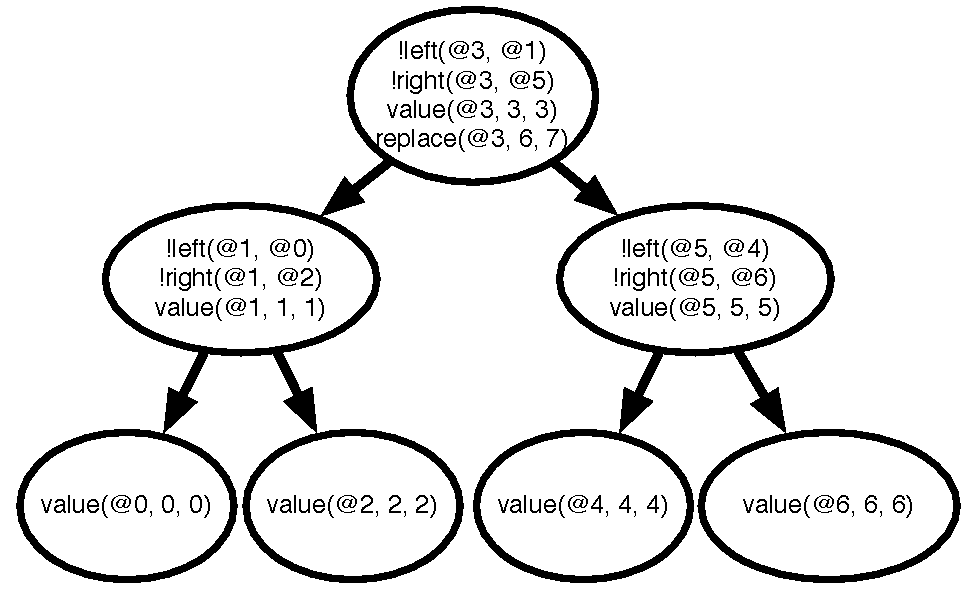
\includegraphics[width=\textwidth]{btree_trace1}
                \caption{Initial database. Replace axiom instantiated at root node $@3$.}
                \label{fig:btree_trace1}
        \end{subfigure}%
        ~
        \begin{subfigure}[b]{0.5\textwidth}
                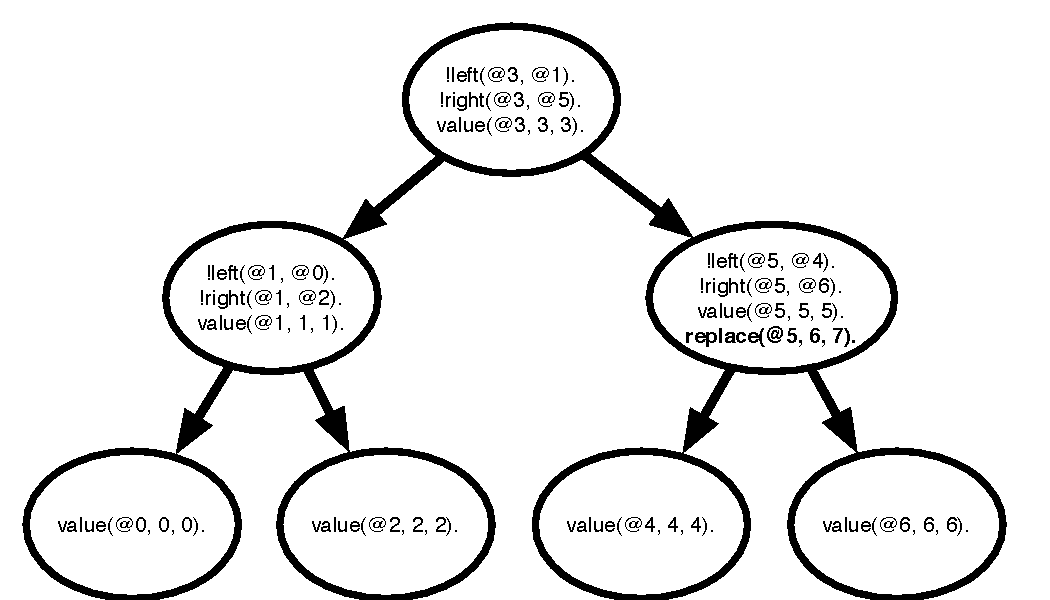
\includegraphics[width=\textwidth]{btree_trace2}
                \caption{After applying rule 3 at node $@3$. Replace fact sent to node $@5$.}
                \label{fig:btree_trace2}
        \end{subfigure}\\
        \begin{subfigure}[b]{0.5\textwidth}
                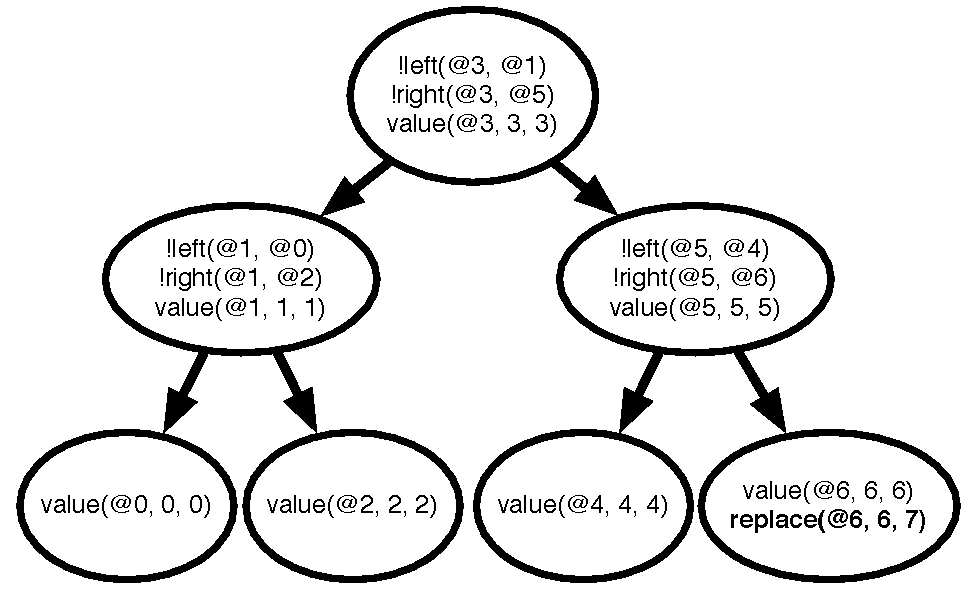
\includegraphics[width=\textwidth]{btree_trace3}
                \caption{After applying rule 3 at node $@5$. Replace fact reaches node $@6$.}
                \label{fig:btree_trace3}
        \end{subfigure}%
        ~
        \begin{subfigure}[b]{0.5\textwidth}
                  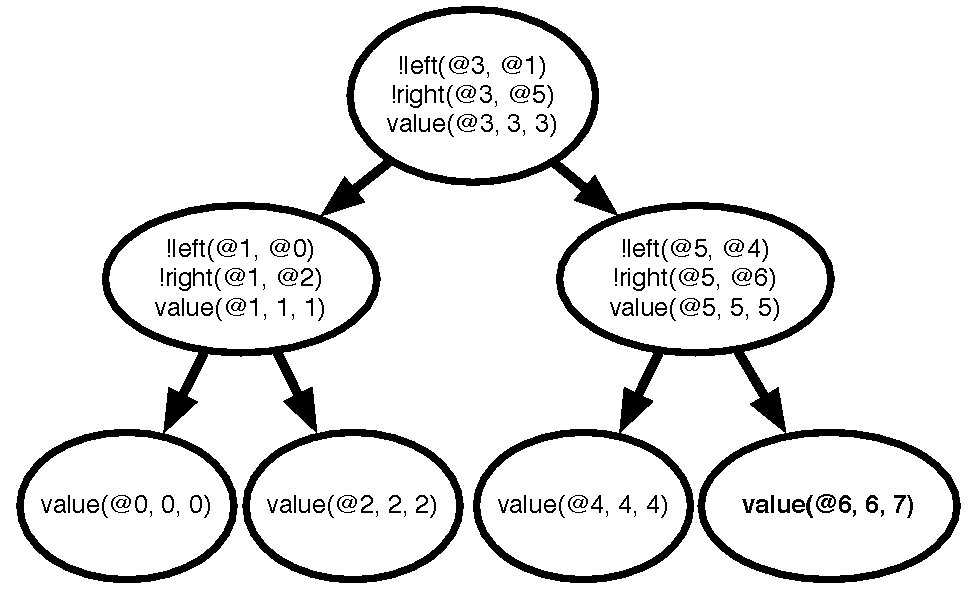
\includegraphics[width=\textwidth]{btree_trace4}
                  \caption{After applying rule 1 at node $@6$. Value of key 6 has changed to 7.}
                  \label{fig:btree_trace4}
          \end{subfigure}
        \caption{An execution trace for the binary tree dictionary algorithm.}\label{fig:btree_trace}
        \vspace{-1.3\intextsep}
\end{figure}

\subsection{Syntax}

\renewcommand{\arraystretch}{1.2}
\begin{table}[h]
\centering
\begin{tabular}{ l l c l }
  Program & $Prog$ & $::=$ & $\Sigma, D$ \\
  Set Of Rules & $\Sigma$ & $::=$ & $\cdot \; | \; \Sigma, R$\\
  Database & $D$ & $::=$ & $\Gamma; \Delta$ \\
  Rule & $R$ & $::=$ & $BE \lolli HE \; | \; \forall_{x}. R$ \\
  Body Expression & $BE$ & $::=$ & $L \; | \; P \; | \; C \; | \; BE, BE \; | \; \exists_{x}. BE \; | \; 1$\\
  Head Expression & $HE$ & $::=$ & $L \; | \; P \; | \; HE, HE \; | \; CE \; | \; AE \; | \; 1$\\
  
  Linear Fact & $L$ & $::=$ & $l(\hat{x})$\\
  Persistent Fact & $P$ & $::=$ & $\bang p(\hat{x})$\\
  Constraint & $C$ & $::=$ & $c(\hat{x})$ \\
  
  Comprehension & $CE$ & $::=$ & $\comprehension$ \\
  Aggregate & $AE$ & $::=$ & $\aggregate$ \\
  Aggregate Operation & $A$ & $::=$ & $\mathtt{min} \; | \; \mathtt{max} \; | \; \mathtt{sum} \; | \; \mathtt{count}$ \\
  
  Sub-Head & $SH$ & $::=$ & $L \; | \; P \; | \; SH, SH \; | \; 1$\\
  
  Known Linear Facts & $\Delta$ & $::=$ & $\cdot \; | \; \Delta, l(\hat{t})$ \\
  Known Persistent Facts & $\Gamma$ & $::=$ & $\cdot \; | \; \Gamma, \bang p(\hat{t})$ \\
\end{tabular}
\vspace{0.5\intextsep}
\caption{Abstract syntax of LM.}
\label{tbl:ast}
\vspace{-1\intextsep}
\end{table}
\renewcommand{\arraystretch}{1.0}

Table~\ref{tbl:ast} shows the abstract syntax for rules in LM.
A LM program $Prog$ consists of a set of derivation rules $\Sigma$ and a database $D$.
Each derivation rule $R$ can be written as $BE \lolli HE$ where $BE$ is the body of a rule and
$HE$ is the head. Rules without bodies are allowed in LM and they are called \textit{axioms}. Rules without heads are also allowed.
The body of a rule, $BE$, may contain linear ($L$) and persistent ($P$) \emph{fact expressions}
and constraints ($C$). Fact expressions are template facts that instantiate variables
(from facts in the database). Variables can be used again in the body for matching and
also in the head when instantiating facts. Constraints are boolean expressions that must
be true in order for the rule to be fired. Constraints use variables from fact expressions and are built using a small functional language that includes mathematical operations, boolean operations, external functions and literal values.
The head of a rule, $HE$, contains linear ($L$) and persistent ($P$) \emph{fact templates} which are uninstantiated facts to derive new facts. The head can also have \emph{comprehensions} ($CE$) and \emph{aggregates} ($AE$). Head
expressions may use the variables instantiated in the body.

\subsubsection{Comprehensions}

Sometimes we need to consume a linear fact and then immediately generate several facts depending on
the contents of the database. To solve this particular need, we created the concept of comprehensions, which are
sub-rules that are applied with all possible combinations of facts from the database. In a comprehension $\comprehension$,
$\widehat{x}$ is a list of variables, $BE$ is the body of the comprehension and $SH$ is the head.
The body $BE$ is used to generate all possible combinations for the head $SH$, according to the facts
in the database.

The following example illustrates a simple program that uses comprehensions:

{\footnotesize
\begin{Verbatim}
!edge(@1, @2).
!edge(@1, @3).
iterate(@1).
iterate(A) -o {B | !edge(A, B) | perform(B)}.
\end{Verbatim}
}

When the rule is fired, we consume \texttt{iterate(@1)} and then generate the comprehension. Here, we iterate through
all the \texttt{edge/2} facts that match \texttt{!edge(@1, B)}, which are: \texttt{!edge(@1, @2)} and \texttt{!edge(@1, @3)}.
For each fact, we derive \texttt{perform(B)}, namely: \texttt{perform(@2)} and \texttt{perform(@3)}.

\subsubsection{Aggregates}

Another useful feature in logic programs is the ability to reduce several facts into a single fact.
In LM we have aggregates ($AE$), a special kind of sub-rule that works very similarly to comprehensions.
In the abstract syntax $\aggregate$, $A$ is the aggregate operation, $\widehat{x}$ is the list of variables
introduced in $BE$, $SH_1$ and $SH_2$ and $y$ is the variable in the body
$BE$ that represents the values to be aggregated using $A$. Like comprehensions,
we use $\widehat{x}$ to try all the combinations of $BE$, but, in addition to deriving $SH_1$ for each combination,
we aggregate the values represented by $y$ and derive $SH_2$ only once using $y$.
As an example, consider the following program:

{\footnotesize
\begin{Verbatim}
price(@1, 3).
price(@1, 4).
price(@1, 5).
count-prices(@1).
count-prices(A) -o [sum => P | . | price(A, P) | 1 | total(A, P)].
\end{Verbatim}
}

By applying the rule, we consume \texttt{count-prices(@1)} and
derive the aggregate which consumes all the \texttt{price(@1, P)} facts.
These are summed and \texttt{total(@1,~12)} is derived.  
LM provides several aggregate operations, including the \emph{minimum}, \emph{maximum}, \emph{sum}, and \emph{count}.

\subsection{Concurrency}

LM is at its core a concurrent programming language.
The database of facts can be seen as a graph data structure where each node contains a fraction of the database.
To accomplish this, we force the first argument of each predicate to be typed as a \emph{node}. We then
restrict the derivation rules to only manipulate facts belonging to a single node.
However, the expressions in the head may refer to other nodes, as long as those nodes are instantiated in the body of the rule.

Due to the restrictions on LM rules, nodes are able to
run rules independently without using other node's facts. Node computation follows a
\emph{don't care} or \emph{committed choice} non-determinism
since any node can be picked to run as long as it contains enough facts to fire a derivation rule.
Facts coming from other nodes will arrive in order of derivation but may be considered
partially and there is no particular order among the neighborhood. To improve concurrency,
the programmer is encouraged to write rules that take advantage of the non-deterministic nature of execution.